\documentclass{beamer}
\usetheme{Antibes}
\usecolortheme{orchid}
\usepackage{amsmath}
\usepackage[utf8]{inputenc}
\usepackage{tikz}
\usepackage{graphicx}
\usepackage{forest}
\usepackage{svg}

\usetikzlibrary{matrix}
\graphicspath{ {./} }

\usepackage{xcolor}

\definecolor{primary}{HTML}{0474E4}
\definecolor{secondary}{HTML}{2185D0}
\definecolor{tertiary}{HTML}{4183C4}
\definecolor{quaternary}{HTML}{384247}
\definecolor{magenta}{HTML}{FF00FF}

\setbeamercolor{palette primary}{bg=primary}
\setbeamercolor{palette secondary}{bg=secondary}
\setbeamercolor{palette tertiary}{bg=tertiary}
\setbeamercolor{palette quaternary}{bg=quaternary}

\setbeamercolor{block title}{fg=primary}
\setbeamercolor{local structure}{fg=primary}

\def\insertauthorindicator{Who?}% Default is "Who?"
\def\insertinstituteindicator{From?}% Default is "From?"
\def\insertdateindicator{When?}% Default is "When?"

\title{Approximate nearest neighbor search using the Hierarchical Navigable Small World (HNSW) algorithm}

\author{Sebastian Bj{\"o}rkqvist}
\institute{Lead AI Developer, IPRally}

\date[12.05.2023]{May 12, 2023}

\newcommand{\kur}{\protect\textit}
\newcommand{\bol}{\protect\textbf}
\newcommand\pro{\item[$+$]}
\newcommand\con{\item[$-$]}

\def\layersep{2.2cm}


\begin{document}
\setbeamertemplate{caption}{\raggedright\insertcaption\par}

\frame{\titlepage}


\begin{frame}
\frametitle{Outline}
  \tableofcontents
\end{frame}
\section{Theoretical foundations}
\subsection{Voronoi diagram}
  \begin{frame}
    \frametitle{Voronoi diagram for a set of points}  
  \begin{figure}[original_points]
    \vspace*{-0.1cm}
  	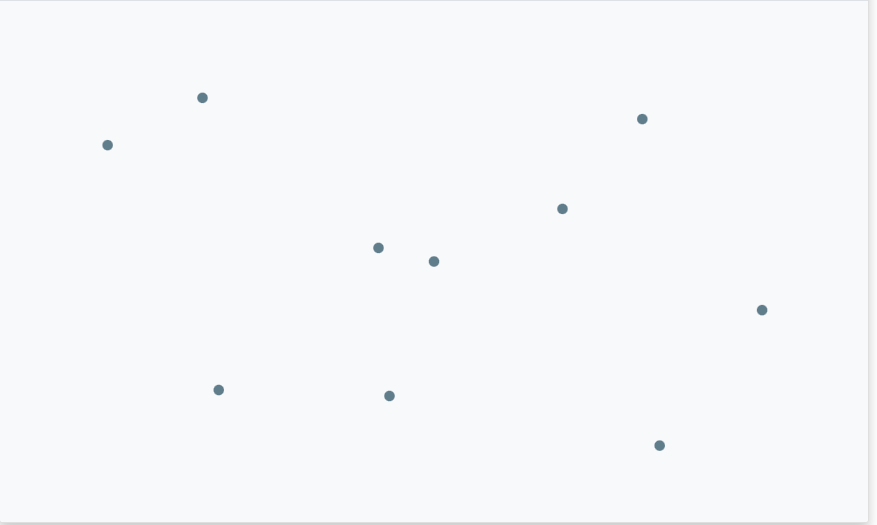
\includegraphics[scale=0.25]{original_points} 	
  \end{figure} 
  \end{frame}
  \begin{frame}
    \frametitle{Voronoi diagram for a set of points}  
  \begin{figure}[voronoi_diagram]
    \vspace*{-0.1cm}
  	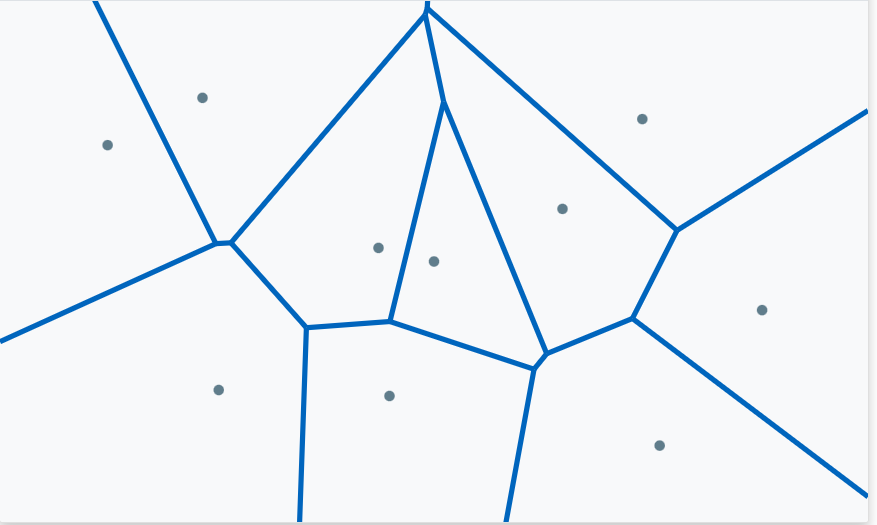
\includegraphics[scale=0.3]{voronoi_diagram} 	
  \end{figure} 
  \end{frame} 

\subsection{Delaunay graph}
  \begin{frame}
    \frametitle{Voronoi diagram to Delaunay graph}  
  \begin{figure}[voronoi_diagram]
    \vspace*{-0.1cm}
  	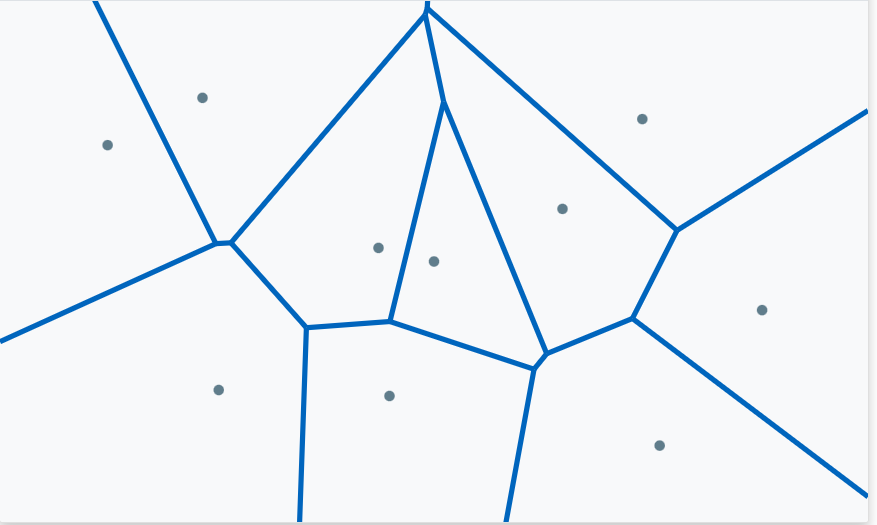
\includegraphics[scale=0.3]{voronoi_diagram} 	
  \end{figure} 
  \end{frame} 

  \begin{frame}
    \frametitle{Voronoi diagram to Delaunay graph}  
  \begin{figure}[voronoi_delaunay]
    \vspace*{-0.1cm}
  	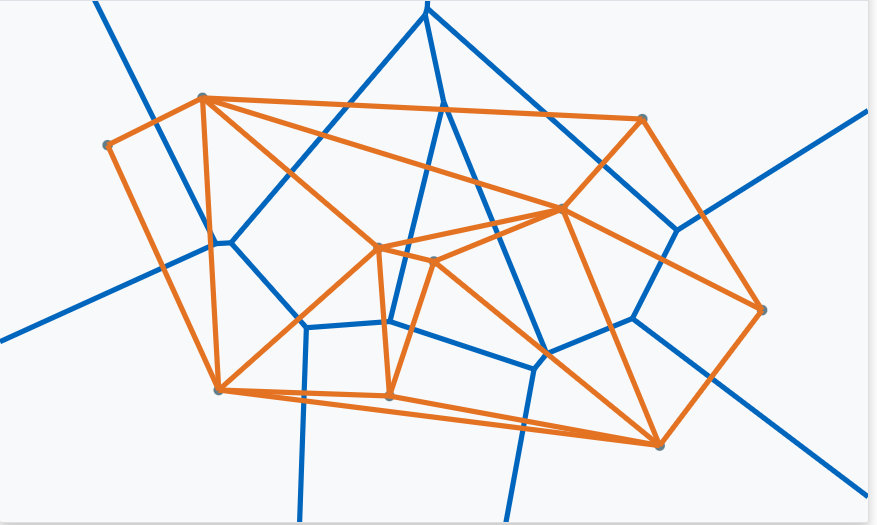
\includegraphics[scale=0.3]{voronoi_delaunay} 	
  \end{figure} 
  \end{frame} 

  \begin{frame}
    \frametitle{Delaunay graph}  
  \begin{figure}[delaunay_graph]
    \vspace*{-0.1cm}
  	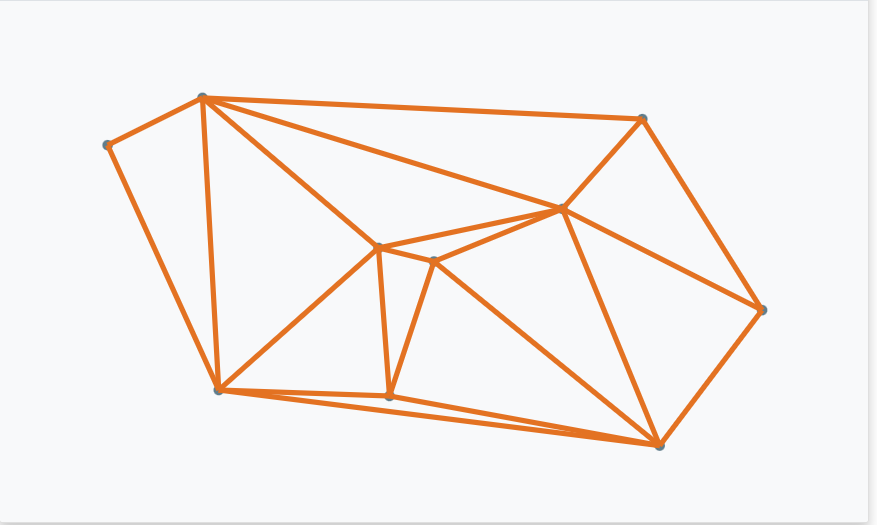
\includegraphics[scale=0.3]{delaunay_graph} 	
  \end{figure} 
  \end{frame} 
  
\subsection{Greedy NN search using Delaunay graph}

  \begin{frame}
    \frametitle{Greedy NN search start - Query and entry point}  
  \begin{figure}[greedy_search_start_new]
    \vspace*{-0.1cm}
  	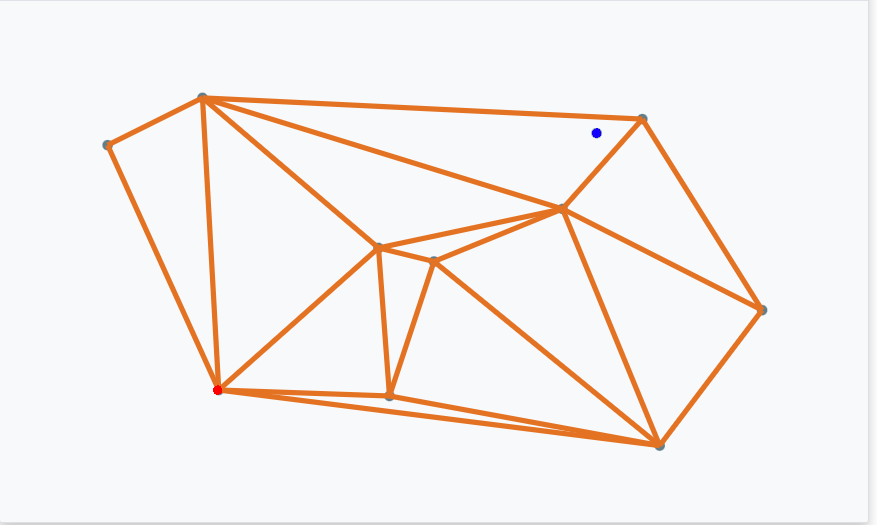
\includegraphics[scale=0.3]{greedy_search_start_new} 	
  \end{figure} 
  \end{frame} 
  

  \begin{frame}
    \frametitle{Greedy NN search - iteration}  
  \begin{figure}[greedy_search_start_new_step_1_1]
    \vspace*{-0.1cm}
  	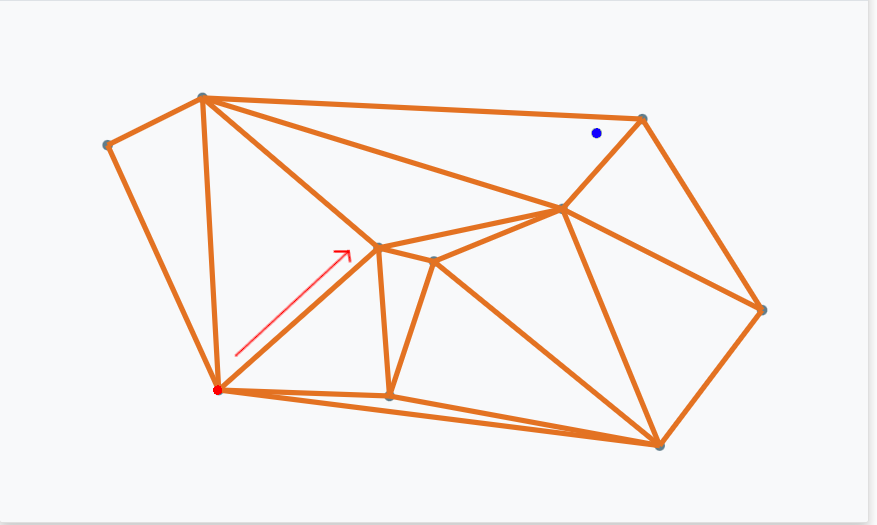
\includegraphics[scale=0.3]{greedy_search_start_new_step_1_1} 	
  \end{figure} 
  \end{frame}   
  

  \begin{frame}
    \frametitle{Greedy NN search - iteration}  
  \begin{figure}[greedy_search_start_new_step_1_2]
    \vspace*{-0.1cm}
  	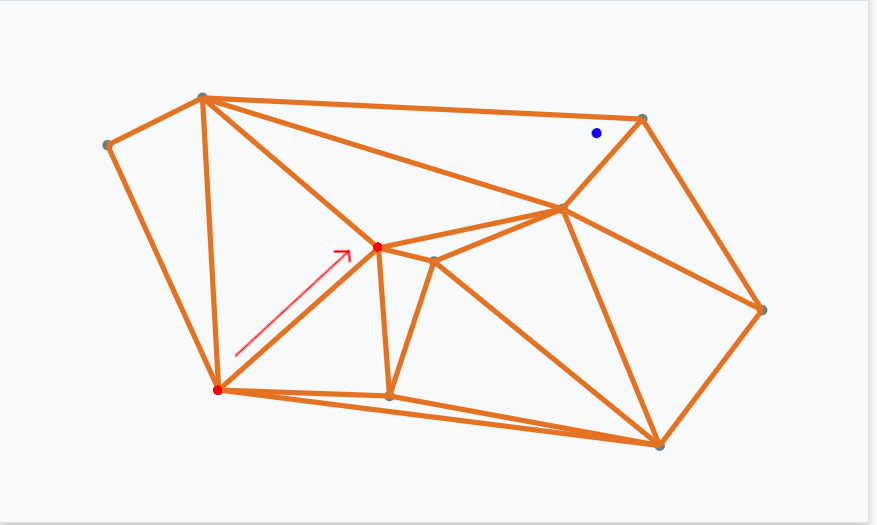
\includegraphics[scale=0.3]{greedy_search_start_new_step_1_2} 	
  \end{figure} 
  \end{frame}     
  

  \begin{frame}
    \frametitle{Greedy NN search - iteration}  
  \begin{figure}[greedy_search_start_new_step_2_1]
    \vspace*{-0.1cm}
  	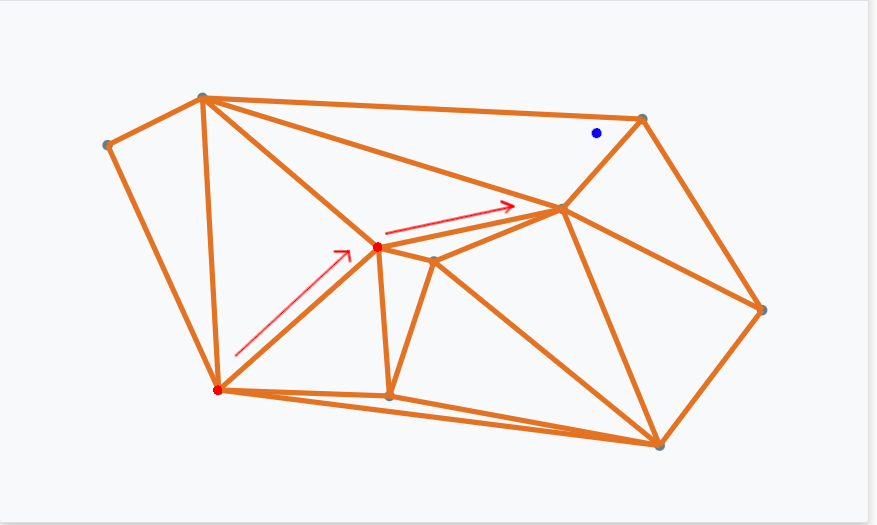
\includegraphics[scale=0.3]{greedy_search_start_new_step_2_1} 	
  \end{figure} 
  \end{frame}       
  
  \begin{frame}
    \frametitle{Greedy NN search - iteration}  
  \begin{figure}[greedy_search_start_new_step_2_2]
    \vspace*{-0.1cm}
  	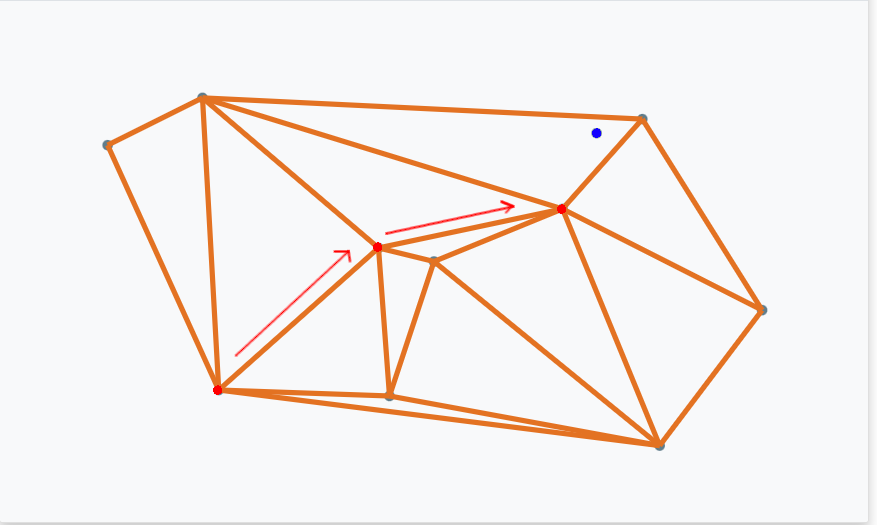
\includegraphics[scale=0.3]{greedy_search_start_new_step_2_2} 	
  \end{figure} 
  \end{frame}         

  \begin{frame}
    \frametitle{Greedy NN search - iteration}  
  \begin{figure}[greedy_search_start_new_step_3_1]
    \vspace*{-0.1cm}
  	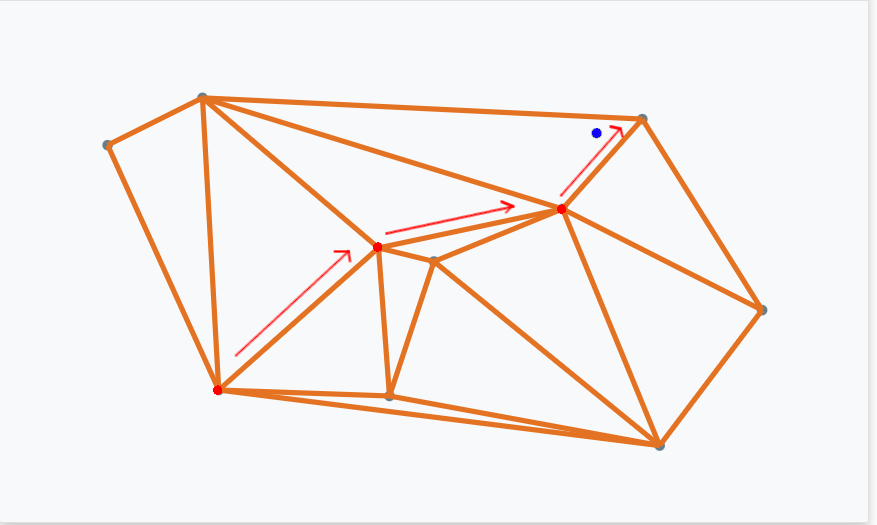
\includegraphics[scale=0.3]{greedy_search_start_new_step_3_1} 	
  \end{figure} 
  \end{frame}         


  \begin{frame}
    \frametitle{Greedy NN search done!}  
  \begin{figure}[greedy_search_start_new_step_3_2]
    \vspace*{-0.1cm}
  	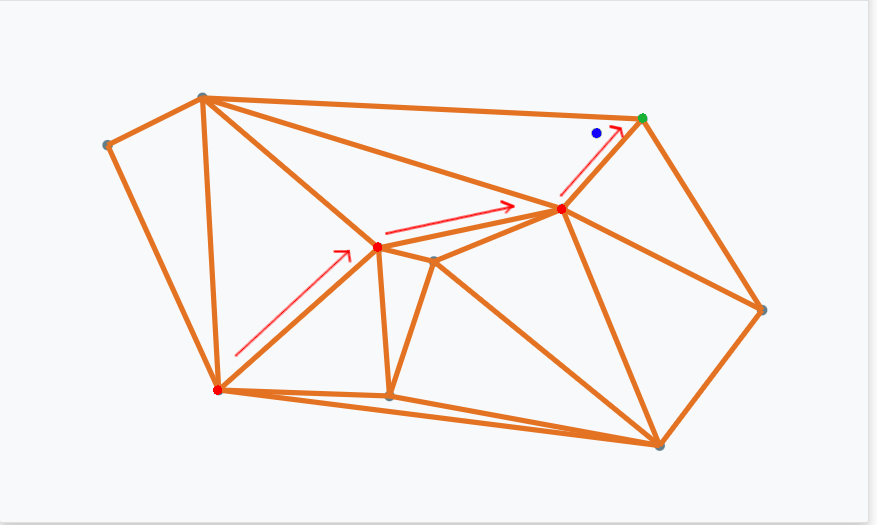
\includegraphics[scale=0.3]{greedy_search_start_new_step_3_2} 	
  \end{figure} 
  \end{frame}         

  \begin{frame}
    \frametitle{Drawbacks}  
   	\begin{itemize}
   	\Large
		\item Delaunay graph intractable to construct for large, high-dimensional data sets
		\item Greedy search might be slow if graph is large
	\end{itemize}   
  \end{frame}

\section{HNSW algorithm}
\subsection{Idea behind algorithm}
  \begin{frame}
    \frametitle{Navigable small world (NSW) graph}  
    \Large
   	\begin{itemize}
   		\onslide<2->{
		\item Small world graph}
		\begin{itemize}
		\onslide<3->{\item Distance of two random nodes is $log \text{ } N$, where $N$ is the number of nodes in graph}
		\onslide<4->{\item Neighbors of a given node are likely to be neighbors of another (clustering coefficient is high)}
		\end{itemize}
		\onslide<5->{		
		\item Navigability}
		\onslide<6->{
		\begin{itemize}
		\item Greedy search algorithm has logarithmic scalability
		\end{itemize}
		}
	\end{itemize}   
  \end{frame}

  \begin{frame}
    \frametitle{Why is an NSW useful for nearest neighbor search?}  
    \Large
    \begin{itemize}
    \onslide<2->{
    \item Logarithmic distance allows us to get anywhere in the graph quickly
    }
    \onslide<3->{
    \item Navigability ensures that the greedy algorithm finds the logaritmic path
    }
    \onslide<4->{
    \item High clustering coefficient lets us zoom in on the actual correct node when we're in the right area
    }
    \end{itemize}
  \end{frame}
  
  \begin{frame}
    \frametitle{Making Delaunay graph navigable}  
          \begin{figure}[delaunay_triangulation_256_points]
  \includesvg[scale=0.5]{delaunay_triangulation_256_points}
  \end{figure}
  \vspace{-0.5cm}
    \centering 256 nodes
  \end{frame}  

  \begin{frame}
    \frametitle{Making Delaunay graph navigable}  
          \begin{figure}[delaunay_triangulation_start_end_points]
  \includesvg[scale=0.5]{delaunay_triangulation_start_end_points}
  \end{figure}
  \end{frame}  

  \begin{frame}
    \frametitle{Making Delaunay graph navigable}  
          \begin{figure}[delaunay_triangulation_longest_path]
  \includesvg[scale=0.5]{delaunay_triangulation_longest_path}
  \end{figure}
  \vspace{-0.5cm}
    \centering Length of path: 19
  \end{frame}  

  \begin{frame}
    \frametitle{Making Delaunay graph navigable}  
          \begin{figure}[delaunay_triangulation_random_edges]
  \includesvg[scale=0.5]{delaunay_triangulation_random_edges}
  \end{figure}
  \vspace{-0.5cm}
    \centering 32 random edges added
  \end{frame}  

  \begin{frame}
    \frametitle{Making Delaunay graph navigable}  
          \begin{figure}[delaunay_triangulation_random_edges_shortest_path]
  \includesvg[scale=0.5]{delaunay_triangulation_random_edges_shortest_path}
  \end{figure}
  \vspace{-0.5cm}
    \centering Length of path: 5
  \end{frame}  


  \begin{frame}
    \frametitle{Properties of NSW graph}  
    \Large
    \onslide<2->{
    \begin{itemize}
    \item An NSW graph is not necessarily a Delaunay graph (or have one as a subgraph)
    }
    \onslide<3->{
    \item Thus the greedy algorithm doesn't always return the actual nearest neighbor
    }
    \onslide<4->{
    \item Ok since we're doing approximate nearest neighbor search!   
    }
    \end{itemize}
  \end{frame}
   

  \begin{frame}
    \frametitle{Constructing NSW graph}  
    \Large
   	\begin{itemize}
   		\onslide<2->{
		\item Approximation of graph is enough (since we're doing approximate nearest neighbor search)}
		\onslide<3->{		
		\item Navigability: Greedy search algorithm has logarithmic scalability
		}
	\end{itemize}   
  \end{frame}

  \begin{frame}
    \frametitle{}  
    \Large How?
   	\begin{itemize}
		\item We can learn a distribution for a document instead of just a single vector
		\item Model prior art relation as KL divergence of distributions
	\end{itemize}   
  \end{frame}

  \begin{frame}
    \frametitle{Distance functions for metadata}  
    \Large Why?
   	\begin{itemize}
		\item We can do soft filtering (by country, patent class etc.)
		\item Can be useful if match is not found by strict filters
	\end{itemize}   
  \end{frame}

  \begin{frame}
    \frametitle{Learning multiple distance functions - naive way}  
\begin{center}
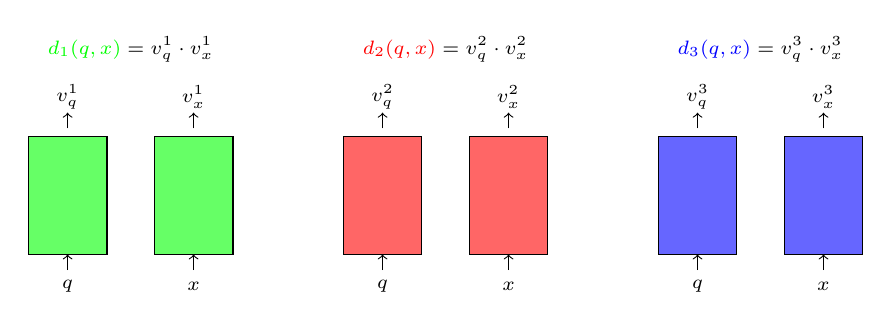
\begin{tikzpicture}[x=2cm, y=2cm]
    \tikzstyle{graphnode}=[circle,fill=black!14,minimum size=2pt,inner sep=0pt]

    \draw[fill=green!60] (-0.8,1.7) rectangle ++(0.5, 0.75);
    \draw[fill=green!60] (0,1.7) rectangle ++(0.5, 0.75);
    
    \node at (-0.55, 1.5) {\scriptsize $q$};
    \node at (0.25, 1.5) {\scriptsize $x$};    
    \draw[->] (-0.55, 1.6) -> (-0.55, 1.7);
    \draw[->] (0.25, 1.6) -> (0.25, 1.7);    

    \node at (-0.55, 2.7) {\scriptsize $v_{q}^{1}$};
    \node at (0.25, 2.7) {\scriptsize $v_{x}^{1}$};  

    \draw[->] (-0.55, 2.5) -> (-0.55, 2.6);
    \draw[->] (0.25, 2.5) -> (0.25, 2.6);
    
    \node at (-0.15, 3) {\scriptsize $\textcolor{green}{d_{1}(q,x)} = v_{q}^{1} \cdot v_{x}^{1}$};   

\onslide<2->{
    \draw[fill=red!60] (1.2,1.7) rectangle ++(0.5, 0.75);
    \draw[fill=red!60] (2,1.7) rectangle ++(0.5, 0.75);
    
    \node at (1.45, 1.5) {\scriptsize $q$};
    \node at (2.25, 1.5) {\scriptsize $x$};    
    \draw[->] (1.45, 1.6) -> (1.45, 1.7);
    \draw[->] (2.25, 1.6) -> (2.25, 1.7);    

    \node at (1.45, 2.7) {\scriptsize $v_{q}^{2}$};
    \node at (2.25, 2.7) {\scriptsize $v_{x}^{2}$};  

    \draw[->] (1.45, 2.5) -> (1.45, 2.6);
    \draw[->] (2.25, 2.5) -> (2.25, 2.6);
    
    \node at (1.85, 3) {\scriptsize $\textcolor{red}{d_{2}(q,x)} = v_{q}^{2} \cdot v_{x}^{2}$};   
}

\onslide<3->{
    \draw[fill=blue!60] (3.2,1.7) rectangle ++(0.5, 0.75);
    \draw[fill=blue!60] (4,1.7) rectangle ++(0.5, 0.75);
    
    \node at (3.45, 1.5) {\scriptsize $q$};
    \node at (4.25, 1.5) {\scriptsize $x$};    
    \draw[->] (3.45, 1.6) -> (3.45, 1.7);
    \draw[->] (4.25, 1.6) -> (4.25, 1.7);    

    \node at (3.45, 2.7) {\scriptsize $v_{q}^{3}$};
    \node at (4.25, 2.7) {\scriptsize $v_{x}^{3}$};  

    \draw[->] (3.45, 2.5) -> (3.45, 2.6);
    \draw[->] (4.25, 2.5) -> (4.25, 2.6);
    
    \node at (3.85, 3) {\scriptsize $\textcolor{blue}{d_{3}(q,x)} = v_{q}^{3} \cdot v_{x}^{3}$};   
}	
  
  
\end{tikzpicture}
\onslide<4->{Drawback: multiple embeddings of same document must be indexed!}
\end{center} 
  \end{frame}

  \begin{frame}
    \frametitle{Learning multiple distance functions - efficient way}  
\begin{center}
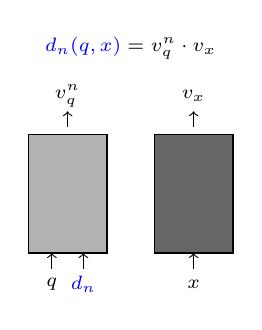
\begin{tikzpicture}[x=2cm, y=2cm]
    \tikzstyle{graphnode}=[circle,fill=black!14,minimum size=2pt,inner sep=0pt]

    \draw[fill=gray!60] (-0.8,1.7) rectangle ++(0.5, 0.75);
    \draw[fill=black!60] (0,1.7) rectangle ++(0.5, 0.75);
    
    \node at (-0.65, 1.5) {\scriptsize $q$};
    \node at (-0.45, 1.5) {\scriptsize $\textcolor{blue}{d_{n}}$};
    \node at (0.25, 1.5) {\scriptsize $x$};    
    \draw[->] (-0.65, 1.6) -> (-0.65, 1.7);
    \draw[->] (-0.45, 1.6) -> (-0.45, 1.7);
    \draw[->] (0.25, 1.6) -> (0.25, 1.7);    

    \node at (-0.55, 2.7) {\scriptsize $v_{q}^{n}$};
    \node at (0.25, 2.7) {\scriptsize $v_{x}$};  

    \draw[->] (-0.55, 2.5) -> (-0.55, 2.6);
    \draw[->] (0.25, 2.5) -> (0.25, 2.6);
    
    \node at (-0.15, 3) {\scriptsize $\textcolor{blue}{d_{n}(q,x)} = v_{q}^{n} \cdot v_{x}$};   


  
  
\end{tikzpicture}
\end{center} 
\begin{center}
\onslide<2->{Only one meta-embedding per document is indexed!}
\end{center}
  \end{frame}

\subsection{Construction of search index}

  \begin{frame}
    \frametitle{Forward thinking} 
  \begin{figure}[original_points]
    \vspace*{-0.1cm}
  	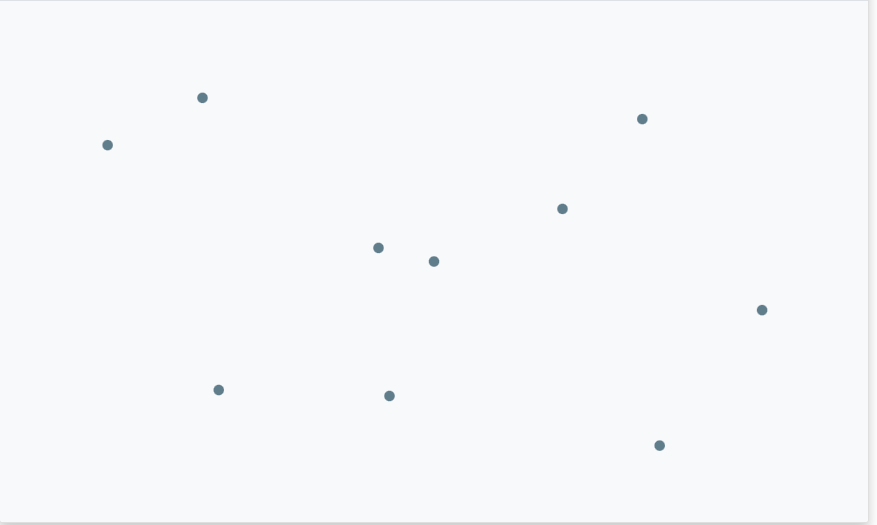
\includegraphics[scale=0.3]{original_points} 	
  \end{figure} 
  \end{frame}    


  \begin{frame}
    \frametitle{Forward thinking} 
    \Large Why?
   	\begin{itemize}
		\item We can train deeper models but keep batch size the same
		\item Training of deep models can take less wall clock time
	\end{itemize}
  \end{frame}    
  
  \begin{frame}
    \frametitle{Forward thinking - paper}  
   	\begin{itemize}
		\item Forward Thinking: Building and Training Neural Networks One Layer at a Time
 (Hettinger et al.) \url{https://arxiv.org/abs/1706.02480}
	\end{itemize}   
  \end{frame}  
  
\subsection{Nearest neighbor search using index}

  \section{Performance}
\subsection{Search accuracy}
  
  \begin{frame}
    \frametitle{Current method - using gradients} 
\begin{center}
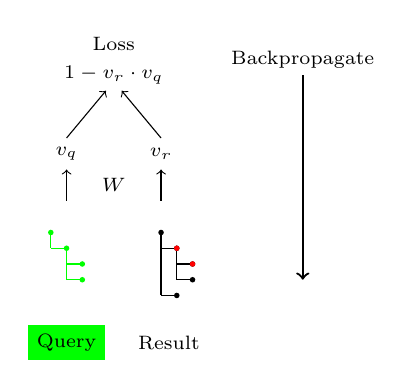
\begin{tikzpicture}[x=2cm, y=2cm]
    \tikzstyle{graphnode}=[circle,fill=black!14,minimum size=2pt,inner sep=0pt]


    \node[fill=green] at (0.2, 1.3) {\scriptsize Query};
    \node at (0.85, 1.3) {\scriptsize Result};    
	
	\node[graphnode, fill=black] at (0.8, 2) {};
    \node[graphnode, fill=black] at (0.9, 1.9) {};
    \node[graphnode, fill=black] at (1, 1.8) {};    
    \node[graphnode, fill=black] at (1, 1.7) {};    
    \node[graphnode, fill=black] at (0.9, 1.6) {};    
	\draw (0.8, 2) -- (0.8, 1.6);
	\draw (0.8, 1.9) -- (0.9, 1.9);	
	\draw (0.9, 1.9) -- (0.9, 1.7);
	\draw (0.9, 1.8) -- (1, 1.8);	
    \draw (0.9, 1.7) -- (1, 1.7);	
    \draw (0.8, 1.6) -- (0.9, 1.6);		
    

	\node[graphnode, fill=green] at (0.1, 2) {};
    \node[graphnode, fill=green] at (0.2, 1.9) {};
    \node[graphnode, fill=green] at (0.3, 1.8) {};    
    \node[graphnode, fill=green] at (0.3, 1.7) {};   
	\draw[green] (0.1, 2) -- (0.1, 1.9);
	\draw[green] (0.1, 1.9) -- (0.2, 1.9);	
	\draw[green] (0.2, 1.9) -- (0.2, 1.7);
	\draw[green] (0.2, 1.8) -- (0.3, 1.8);	
    \draw[green] (0.2, 1.7) -- (0.3, 1.7);		
    
    
    \onslide<2->{
    \draw[->] (0.8, 2.2) -> (0.8, 2.4);
    \draw[->] (0.2, 2.2) -> (0.2, 2.4);
    

    \node at (0.8, 2.5) {\scriptsize $v_{r}$};
    \node at (0.5, 2.3) {\scriptsize $W$};
    \node at (0.2, 2.5) {\scriptsize $v_{q}$};  
    }
    
    \onslide<3->{
    
    \draw[->] (0.2, 2.6) -> (0.45, 2.9);
    \draw[->] (0.8, 2.6) -> (0.55, 2.9);
    
    \node at (0.5, 3) {\scriptsize $1 - v_{r} \cdot v_{q}$};
    \node at (0.5, 3.2) {\scriptsize Loss};
    }
    
    \onslide<4->{
    \draw[->, thick] (1.7, 3) -> (1.7, 1.7); 
    \node at (1.7, 3.1) {\scriptsize Backpropagate};
    }
    \onslide<5->{
    \node[graphnode, fill=red] at (0.9, 1.9) {};
    \node[graphnode, fill=red] at (1, 1.8) {};     
    }
      
  
\end{tikzpicture}
\end{center}	

\onslide<5->{Nodes with highest gradient are considered most important
}
  \end{frame}     
  
  \begin{frame}
    \frametitle{Drawbacks with using gradients} 
   	\begin{itemize}
		\item Compute-intensive, since we need to do backwards pass
		\item Quality of explanations is not the best
		\begin{itemize}
		\item Evaluating Recurrent Neural Network Explanations (Arras et al.) \url{https://arxiv.org/abs/1904.11829}
		\end{itemize}
	\end{itemize}
  \end{frame}     
  
  \begin{frame}
    \frametitle{Comparing node embeddings} 
  \begin{figure}[node_embedding_comparison]
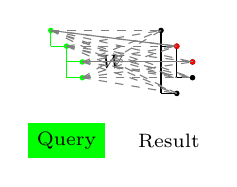
\begin{tikzpicture}[x=2cm, y=2cm]
    \tikzstyle{graphnode}=[circle,fill=black!14,minimum size=2pt,inner sep=0pt]


    \node[fill=green] at (0.2, 1.3) {\scriptsize Query};
    \node at (0.85, 1.3) {\scriptsize Result};    
	
	\node[graphnode, fill=black] at (0.8, 2) {};
    \node[graphnode, fill=black] at (0.9, 1.9) {};
    \node[graphnode, fill=black] at (1, 1.8) {};    
    \node[graphnode, fill=black] at (1, 1.7) {};    
    \node[graphnode, fill=black] at (0.9, 1.6) {};    
	\draw (0.8, 2) -- (0.8, 1.6);
	\draw (0.8, 1.9) -- (0.9, 1.9);	
	\draw (0.9, 1.9) -- (0.9, 1.7);
	\draw (0.9, 1.8) -- (1, 1.8);	
    \draw (0.9, 1.7) -- (1, 1.7);	
    \draw (0.8, 1.6) -- (0.9, 1.6);		
    

	\node[graphnode, fill=green] at (0.1, 2) {};
    \node[graphnode, fill=green] at (0.2, 1.9) {};
    \node[graphnode, fill=green] at (0.3, 1.8) {};    
    \node[graphnode, fill=green] at (0.3, 1.7) {};   
	\draw[green] (0.1, 2) -- (0.1, 1.9);
	\draw[green] (0.1, 1.9) -- (0.2, 1.9);	
	\draw[green] (0.2, 1.9) -- (0.2, 1.7);
	\draw[green] (0.2, 1.8) -- (0.3, 1.8);	
    \draw[green] (0.2, 1.7) -- (0.3, 1.7);		
    
    
    \onslide<2>{
    \node at (0.5, 1.8) {\scriptsize $W$};
    }
    \onslide<3>{
    \draw[dashed,gray] (0.1, 2) -- (0.8, 2);
    \draw[dashed,gray] (0.1, 2) -- (0.9, 1.9);     
    \draw[dashed,gray] (0.1, 2) -- (0.9, 1.7);        
    \draw[dashed,gray] (0.1, 2) -- (1, 1.8);          
    \draw[dashed,gray] (0.1, 2) -- (1, 1.7);            
    \draw[dashed,gray] (0.1, 2) -- (0.9, 1.6);  
    \draw[dashed,gray] (0.2, 1.9) -- (0.8, 2);
    \draw[dashed,gray] (0.2, 1.9) -- (0.9, 1.9);     
    \draw[dashed,gray] (0.2, 1.9) -- (0.9, 1.7);        
    \draw[dashed,gray] (0.2, 1.9) -- (1, 1.8);          
    \draw[dashed,gray] (0.2, 1.9) -- (1, 1.7);            
    \draw[dashed,gray] (0.2, 1.9) -- (0.9, 1.6);             
    \draw[dashed,gray] (0.3, 1.8) -- (0.8, 2);
    \draw[dashed,gray] (0.3, 1.8) -- (0.9, 1.9);     
    \draw[dashed,gray] (0.3, 1.8) -- (0.9, 1.7);        
    \draw[dashed,gray] (0.3, 1.8) -- (1, 1.8);          
    \draw[dashed,gray] (0.3, 1.8) -- (1, 1.7);            
    \draw[dashed,gray] (0.3, 1.8) -- (0.9, 1.6);           
    \draw[dashed,gray] (0.3, 1.7) -- (0.8, 2);
    \draw[dashed,gray] (0.3, 1.7) -- (0.9, 1.9);     
    \draw[dashed,gray] (0.3, 1.7) -- (0.9, 1.7);        
    \draw[dashed,gray] (0.3, 1.7) -- (1, 1.8);          
    \draw[dashed,gray] (0.3, 1.7) -- (1, 1.7);            
    \draw[dashed,gray] (0.3, 1.7) -- (0.9, 1.6);     
    }
    
    \onslide<4>{
    \node[graphnode, fill=red] at (0.9, 1.9) {};
    \node[graphnode, fill=red] at (1, 1.8) {};     
    \draw[gray] (0.1, 2) -- (0.9, 1.9);     
    \draw[gray] (0.3, 1.8) -- (1, 1.8);          
    
    }    
          
  
\end{tikzpicture}
\end{figure}
\begin{center}
\begin{enumerate}
\onslide<2->{
\item Embed graphs using model
}
\onslide<3->{
\item Compare each pair of node embeddings
}
\onslide<4->{
\item Highlight most similar nodes
}
\end{enumerate}
\end{center}

  \end{frame}        

  \begin{frame}
    \frametitle{Comparing node embeddings}  
    \Large Why?
   	\begin{itemize}
		\item Faster than using gradients (no backprop step needed)
		\item Might give more relevant explanations
		\item Can be useful for finding missing features
	\end{itemize}   
  \end{frame}



\subsection{Build time}

\section{}
  \begin{frame}
    \frametitle{References}  
    \small
    \begin{itemize}
	\item \textit{Efficient and robust approximate nearest neighbor search using Hierarchical Navigable Small World graphs (Malkov et al.} \url{https://arxiv.org/abs/1603.09320}    

	\item \textit{Approximate nearest neighbor algorithm based on navigable small world graphs (Malkov et al} \url{https://doi.org/10.1016/j.is.2013.10.006}	
	\item \textit{Voronoi diagrams—a survey of a fundamental geometric data structure (Aurenhammer)} \url{https://dl.acm.org/doi/10.1145/116873.116880}
	\item \textit{Hierarchical Navigable Small Worlds (HNSW) (Pinecone blog)} \url{https://www.pinecone.io/learn/hnsw/}
	\end{itemize}
	
  \end{frame}



\end{document}
